\section{Results and discussion}

Test prints were performed on an unmodified Ultimaker S5 system,
with a standard  \SI{0.4}{\milli\meter} nozzle
and PLA filament
and a layer thickness of $h=\SI{0.1}{\milli\meter}$.
In order to accurately realize a varying bead width we vary the movement speed, while keeping the internal pressure in the system constant.
One approach would be keep the filament inflow $f$ (in \si{\milli\meter\cubed\per\second}) constant by varying movement speed accordingly.
However, that doesn't result in the intended filament outflow variation - see \cref{zero_backpressure}.
We conjecture that the filament outflow is related to the total pressure in the system,
which depends not only on the amount of filament in between the feeder wheel and the nozzle (which we keep constant), 
but also depends on the backpressure that the previous layer exerts on the filament protruding from the nozzle.
We conjecture that the amount of backpressure is monotonically related to the requested line width and compensate for the backpressure using a simple linear model:

\begin{align}
 v(w) &= \frac{f(w)}{h w} \\ 
% f &\sim p \\
% p &= p_\text{in} + p_\text{ext} \\
% p_\text{in} &= C \\
% p_\text{ext} &\sim w \\
% p_\text{ext} &= w / w^* - 1 \\
% f &= f^* - k p_\text{ext} \\
 f(w) &= f_0 - k \left( w / w_0 - 1 \right) \\
 f_0 &= v_0 w_0 h 
% v &= \frac{f^* - k p_\text{ext}}{h w} \\ 
% v &= \frac{v^* w^* h - k (w / w^* - 1)}{h w}
\end{align}
where
$v(w)$ is the movement speed as a function of requested bead width $w$,
$f(w)$ is the filament outflow,
$f_0$ is a constant reference flow
and
$k$ is the amount of backpressure compensation.
Using increments of $0.1$ we established that using a factor of $k=1.1$ yields satisfactory bead width variation for our setup where
$v_0=\SI{30}{\milli\meter\per\second}$, 
$w_0=\SI{0.4}{\milli\meter}$.
See \cref{backpressure}.

\begin{figure}
\centering
\setlength{\figwidth}{0.32\columnwidth}
\setlength{\figheight}{0.5\columnwidth}
\begin{subfigure}[t]{\figwidth}\centering
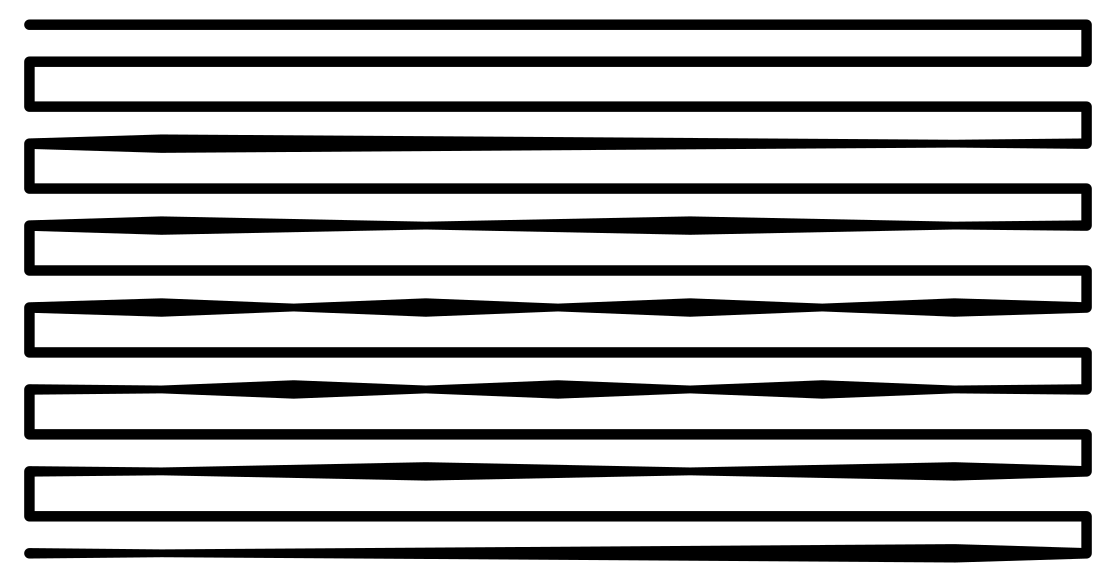
\includegraphics[angle=90,height=\figheight]{sources-validation-backpressure-compensation-target.pdf}
\caption{Target widths}\label{backpressure_target}
\end{subfigure}
\begin{subfigure}[t]{\figwidth}\centering
\includegraphics[angle=90,height=\figheight]{sources-validation-zero-backpressure-compensation.png}
\caption{Constant filament inflow (\si{\milli\meter\cubed\per\second})}\label{zero_backpressure}
\end{subfigure}
\begin{subfigure}[t]{\figwidth}\centering
\includegraphics[angle=90,height=\figheight]{sources-validation-backpressure-compensation.png}
\caption{Backpressure compensation}\label{backpressure}
\end{subfigure}
\caption{
Print results of varying width test on top of a dense white raft.
Trying to reproduce \subref{backpressure_target} without backpressure compensation ($k=0$) yields worse results \subref{zero_backpressure} than with backpressure compensation $k=1.1$ \subref{backpressure}.
}
\label{backpressure_compensation}
\end{figure}


% adapted from 5.5 Discussion on implications
\todo{Reword the following paragraph, which is adapted from 5.5 Discussion on implications.}

Note that the current industry standard in FDM printing employs little to no bead width variation.
\revise{
Properly performing bead width variation calls for adaptations and developments in printers and firmware.
In the beading schemes we set a transition length of $t(n) = w^*$.
That will demand changes in cross-sectional area of the bead up to \SI{200}{\percent} over a small distance that is comparable to the nozzle size, which is challenging for some hardware systems.
Varying the movement speed can be utilized to change the cross-sectional area, 
}{While some software packages generate toolpaths similar to the state-of-the-art,
the naive constant width offset approach is still widely used.
Our backpressure compensation algorithm effectively changes the speed to realize adaptive width,
}
but this approach is limited, since the movement speed is constrained by acceleration considerations near bends in the toolpath~\cite{Ertay2018,Kuipers2018}.
\revise{
Our schemes require a more accurate control of the volumetric flow rate in \si{\milli\meter\cubed\per\second}.
}{}
Using a filament feeder directly mounted on the print head (a.k.a. direct drive) can \revise{control the flow more dynamicaly}{provide more dynamic control over the flow} \revise{then}{than} FDM printers where the material is fed through a Bowden tube from a feeder mounted on the frame.
\revise{
Still direct drive printers require some control system in order to accurately change the volumetric flow rate such as pressure advance algorithms~\cite{tronvoll2019investigating}.
Yet inaccuracies in direct drive systems employing advance algorithms might arise due to the changes in back-pressure required by changing bead size.
We expect that developments in printing hardware and firmware will address these challenges in the future.
}{Direct drive printers can benefit from \emph{pressure advance algorithms} which dynamically change the internal pressure \cite{tronvoll2019investigating},
but presumably backpressure would still be a significant factor one might want to compensate for.
}


\todo{For super small layer heights it might be impossible to reach a bead width range with a factor of $2$.}

Another limiting factor for adopting adaptive bead width is the format of G-code which stores machine instructions.
G-code does not support moves with varying cross-sectional area.
A typical extrusion move \lstinline{G1 X$x$ Y$y$ E$v$} only specifies the total amount of volume $v$ to be extruded in the move, not how that total amount should be distributed along the extrusion move.
A workaround is to approximate a variable width extrusion segment by smaller segments with constant width.
However, this introduces errors nevertheless.
Ideally the G-code language would be expanded in some way to allow for extrusion segments with varying cross-sectional area.





{
\subsection{Computational results}\label{sec_computational_results}
} % tew
We evaluate the proposed framework and the various beading schemes on a set of different types of 3D models, ranging over various applications and various types of geometry. 
The data set is described in Appendix~\ref{dataset}.
We sliced all models in the data set and selected 300 random slices for analysis.
Toolpaths of these 300 outline shapes are generated using the uniform technique as implemented by Clipper~\cite{johnson2014clipper} -- a state-of-the-art polygon offset library,
and by our framework using four beading schemes, i.e. the constant bead count scheme with a bead count of $C=4$, the centered, the evenly distributed, and the inward distributed beading scheme using {$N=2$}, all with a preferred bead width{} of {$w^* = \SI{0.5}{\milli\meter}$ and using the widening meta-scheme to enforce a minimum printed feature size of $w_\text{min}=2r_\text{min}=\SI{0.3}{\milli\meter}$}.
The tests were performed on a desktop PC equipped with an Intel Core i7-7500U CPU @ \SI{2.70}{\giga\hertz} (a single core is used) and \SI{16.3}{\giga\byte} memory.
{We report on the total statistics summed over the whole data set, because averaging would be biased.}






\subsubsection{Accuracy}
We first evaluate the accuracy of different beading schemes in terms of the relative amount of the overfill and underfill. 
We construct the over- and underfill area by comparing the shapes covered by each extrusion move  with each other and with the total shape of the boundary polygons. (For implementation details see Appendix~\ref{accuracy_calculation}.)
This results in polygonal shapes such as visualized in the top half of \cref{visualized_accuracy}:
there are orange shapes where the beads overlap and azure shapes in the voids in between the beads.
%
%
We compare the total area in \si{\milli\meter\squared} of these overfill and underfill shapes to the total area of the boundary for each sample in the data set
and report the average percentages in \cref{over_underfill}.
The inward distributed scheme has a calculated overfill of {\SI{0.30}{\percent}} and an underfill of {\SI{0.24}{\percent}}.
This is lower compared to the uniform scheme, which results in {\SI{1.63}{\percent}} overfill and {\SI{1.62}{\percent}} underfill in the data set.
\iffalse
names ['naive', 'Constant', 'Center', 'Distributed', 'InwardDistributed']
overfill [  1.63223926  22.21073295   0.37059604   0.45119725   0.30226112]
outer_underfill [ 0.04664107  0.03232884  0.04357603  0.03494708  0.03475748]
underfill [ 1.62009421  0.0712721   0.76886316  0.2440984   0.24461937]
\fi

\begin{figure*}
\centering
\setlength{\figwidth}{0.19\textwidth}
\setlength{\figheight}{0.283\textwidth}
\begin{subfigure}{\figwidth}\centering
\includegraphics[height=\figheight]{sources-validation-gMAT-example-TEST-naive-accuracy.png}
\includegraphics[height=\figheight]{sources-validation-gMAT-example-TEST-naive-widths.png}
\caption{Uniform}\label{TEST_naive_accuracy}
\end{subfigure}
%\begin{subfigure}{\figwidth}\centering
%\includegraphics[height=\figheight]{sources-validation-gMAT-example-TEST-SingleBead-accuracy.png}
%\includegraphics[height=\figheight]{sources-validation-gMAT-example-TEST-SingleBead-widths.png}
%\caption{Single}\label{TEST_SingleBead_accuracy}
%\end{subfigure}
\begin{subfigure}{\figwidth}\centering
\includegraphics[height=\figheight]{sources-validation-gMAT-example-TEST-Constant-accuracy.png}
\includegraphics[height=\figheight]{sources-validation-gMAT-example-TEST-Constant-widths.png}
\caption{Constant}\label{TEST_Constant_accuracy}
\end{subfigure}
\begin{subfigure}{\figwidth}\centering
\includegraphics[height=\figheight]{sources-validation-gMAT-example-TEST-Center-accuracy.png}
\includegraphics[height=\figheight]{sources-validation-gMAT-example-TEST-Center-widths.png}
\caption{Centered}\label{TEST_Center_accuracy}
\end{subfigure}
\begin{subfigure}{\figwidth}\centering
\includegraphics[height=\figheight]{sources-validation-gMAT-example-TEST-Distributed-accuracy.png}
\includegraphics[height=\figheight]{sources-validation-gMAT-example-TEST-Distributed-widths.png}
\caption{Distributed}\label{TEST_Distributed_accuracy}
\end{subfigure}
\begin{subfigure}{\figwidth}\centering
\includegraphics[height=\figheight]{sources-validation-gMAT-example-TEST-InwardDistributed-accuracy.png}
\includegraphics[height=\figheight]{sources-validation-gMAT-example-TEST-InwardDistributed-widths.png}
\caption{Inward {($N=2$)}}\label{TEST_InwardDistributed_accuracy}
\end{subfigure}
\begin{subfigure}{.04\columnwidth}\centering
\vspace{4.7cm}
\includegraphics[height=\figheight]{sources-validation-gMAT-example-widths-legend.pdf}
\end{subfigure}
\caption{
Visualization of the overfills and underfills (top) and the widths (bottom) for various beading schemes.
Extrusion beads in gray tones,
overfill in orange,
underfill in azure,
narrow beads in blue
and wide beads in red.
{In order to distinguish clearly from the Distributed scheme the Inward is limited to $N=2$.}
}
\label{visualized_accuracy}
\end{figure*}




\begin{figure*}
\centering
\setlength{\figheight}{0.25\textwidth}
\setlength{\figwidth}{0.32\textwidth}
\begin{subfigure}{\figwidth}\centering
\includegraphics[height=\figheight]{sources-validation-over-underfill.pdf}
%\includegraphics[width=\figwidth]{sources-validation-overunderfill.pdf}
\caption{{Over- and underfill}}
\label{over_underfill}
\end{subfigure}
\begin{subfigure}{\figwidth}\centering
\includegraphics[height=\figheight]{sources-validation-print-time.pdf}
%\includegraphics[width=\figwidth]{sources-validation-smoothness.pdf}
\caption{{Print time}}
\label{printtime}
\end{subfigure}
\begin{subfigure}{\figwidth}\centering
\includegraphics[height=\figheight]{sources-validation-path-counts.pdf}
%\includegraphics[width=\figwidth]{sources-validation-widthHistogram.pdf}
\caption{{Path counts}}
\label{pathcounts}
\end{subfigure}

\begin{subfigure}{\figwidth}\centering
\includegraphics[height=\figheight]{sources-validation-widths.pdf}
%\includegraphics[width=\figwidth]{sources-validation-widthHistogram.pdf}
\caption{{Extrusion widths}}
\label{widthHistogram}
\end{subfigure}
\begin{subfigure}{\figwidth}\centering
\includegraphics[height=\figheight]{sources-validation-angles.pdf}
%\includegraphics[width=\figwidth]{sources-validation-smoothnessNoTransition.pdf}
\caption{{Site angles}}
\label{smoothness}
\end{subfigure}
\begin{subfigure}{\figwidth}\centering
\includegraphics[height=\figheight]{sources-validation-computime2.pdf}
%\includegraphics[width=\figwidth]{sources-validation-computime2.pdf}
\caption{Computation time}
\label{computime}
\end{subfigure}


\caption{
Statistical analysis of the toolpaths from applying the uniform width technique and various beading schemes using our framework to a data set of 300 slices.
Note the use of a logarithmic scale {in the bottom graphs }on the Y-axes and {for \subref{computime} on} the X-axes as well.
}
\label{statisticsfig}
\end{figure*}







\subsubsection{Uniformity}
We visualize the bead widths resulting from the different schemes in the bottom of \cref{visualized_accuracy}.
{
We binned the toolpaths into width bins at \SI{0.01}{\milli\meter} increments and determine the total toolpath length pertaining to each bin.
From these statistics we calculate the mean and standard deviation and report them in \cref{widthHistogram}.
}
We found that the mean width of the inward and evenly distributed schemes is close to preferred bead width of \SI{400}{\micro\meter}, while their standard deviation is lower than for the centered and constant bead count scheme. 
These results show that, while causing less overfill and underfill, inwards distributed and evenly distributed schemes deviate less or less often from the preferred bead width compared to the other schemes.


{
\subsubsection{Print time}
The total time it takes to print a part is influenced not only by our back pressure compensation scheme, but also by the geometry of the toolpaths.
In order to separate these effects we report on the total print time when using back pressure compensation and when using a constant (maximum) movement speed in \cref{printtime}.
We estimate print times using a simulation of the Marlin firmware using the default movement settings of the setup described in \cref{print_results_section}.
While the idealized print time is predominantly determined by the total toolpath length, the print time using back pressure compensation is predominantly determined by the occurrence of wide beads, because they have a reduced the flow in \si{\milli\meter\cubed\per\second}.
Because of acceleration constraints imposed by the hardware the maximum movement speed is not reached near sharp corners.
We therefore also report on the angles of the bends in the toolpaths in \cref{smoothness}.
Furthermore, the print time is negatively affected by discontinuities in the extrusion process.
Between extrusions the printer needs to stop extrusion, travel to the next extrusion path and restart the extrusion process, which may introduce defects and incurs extra print time.
For closed polygonal toolpaths we can start anywhere within the path, so we can optimize the starting location so as to minimize the travel time.
We therefore report both on the open and closed path count in \cref{pathcounts}.
}


\subsubsection{Computational performance}
\cref{computime} plots the computation time against the vertex count of the layer for the full data set, comparing the uniform technique implemented using Clipper~\cite{johnson2014clipper} to our framework with the inward distributed scheme.
For polygonal shapes with as many as $10^4$ vertices, the computation for both approaches is less than 1 second, with our method being approximately five times that of the uniform technique.
These results could be improved upon by utilizing the locality inherent in our algorithms for parallelization on the GPU.

The computational complexity is limited by the generation of the Voronoi Diagram, which is $O(n \log n)$, where $n$ is the number of vertices in the input shape.
The other steps in our framework have a complexity of $O(m)$, where $m$ is the number of elements in the ST.
Therefore, the total running time of our algorithm is $O(n \log n)$.
Results in \cref{computime} confirm that both our framework and the uniform technique have an expected running time of approximately $5 \times 10^{-6} n \log n$ seconds.















%We therefore visualize include a semi-circle with a diameter equal to the starting width in the one end, and exclude it at the other end, because it will be included in the next extrusion segment.


